\section{Overview}

This very basic tutorial provides and introduction to Bayesian inference and Markov chain Monte Carlo (MCMC) algorithms.
The tutorial explains the fundamental concepts of an MCMC algorithm, such as \emph{moves} and \emph{monitors}, which are ubiquitous in every other tutorial.
After the tutorial you should be somewhat familiar with Bayesian inference (\EG what is a prior distribution, posterior distribution, and likelihood function) and MCMC simulation (\EG what are moves and monitors and why do we need them).

\section{A Coin Flipping (Binomial) Model}

We'll begin our exploration of Bayesian inference with a simple coin-flipping model.
In this model, we imagine flipping a coin $n$ times and count the number of heads, $x$; each flip comes up heads with probability $p$.
This model gives rise to the Binomial probability distribution, with parameters $n$ and $p$:
\begin{align*}
P(x \mid n,p) = {n \choose x}p^x(1-p)^{n-x}
\end{align*}
Simple intuition suggests that, given that we observe $x$ heads in $n$ coin tosses, the maximum-likelihood estimate (MLE) of $p$ is simply $\frac{x}{n}$: if we flip a coin 100 times and observe 70 heads, we assume the probability the coin comes up heads is $\frac{70}{100} = 0.7$.
This is indeed the maximum likelihood estimate!

From Bayes' theorem, the \emph{posterior distribution} of $p$ given $x$, $P(p \mid x)$, is:
\begin{align*}
\overbrace{P(p \mid x)}^{\text{posterior distribution}} = \frac{ \overbrace{P(x \mid p)}^{\text{likelihood}} \times \overbrace{P(x)}^{\text{prior}}}{\underbrace{P(x)}_{\text{marginal likelihood}}}
\end{align*}
The take-home message here is that, if we're interested in doing Bayesian inference for the coin flipping model, we need to specify a \emph{likelihood function} and a \emph{prior distribution} for $p$.
In virtually all practical cases, we cannot compute the posterior distribution directly and instead use numerical procedures, such as a Markov chain Monte Carlo (MCMC) algorithm.
Therefore, we will also have to write an MCMC algorithm that samples parameter values in the frequency of their posterior probability.

We'll use a simple beta distribution as a prior on the parameter of the model, $p$.
The beta distribution has two parameters, $\alpha$ and $\beta$ (Figure 1).
The graphical model for the binomial model is depicted in Figure 2.

\begin{figure}[h!]
\centering
\fbox{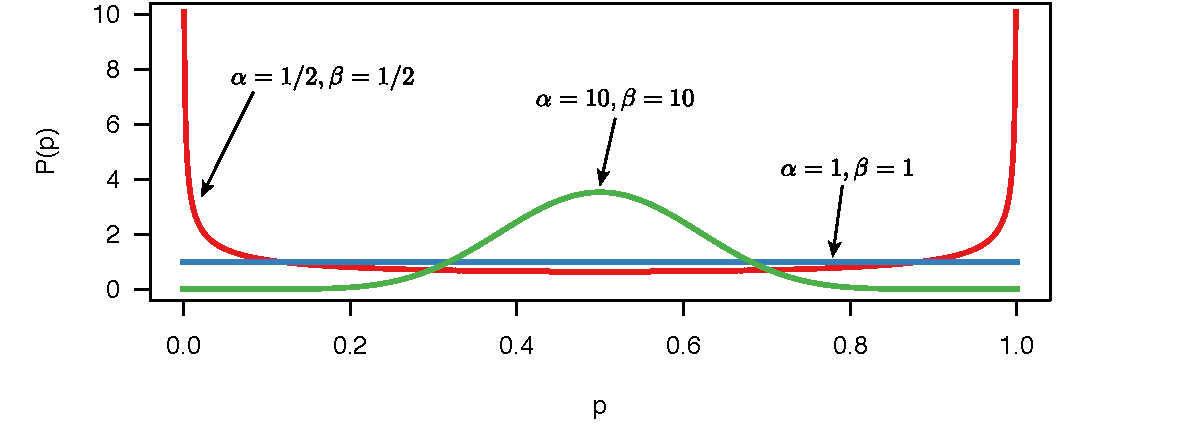
\includegraphics[width=0.7\linewidth,angle=0]{\ResourcePath figures/beta.pdf}}
\label{beta_distribution}
\caption{A beta distribution with two parameters, $\alpha$ and $\beta$. This distribution is used as a prior distribution on the probability parameter $p$ of observing a head. Here we show different curves for the beta distribution when using different parameters.}
\end{figure}

\begin{figure}[h!]
\centering
\fbox{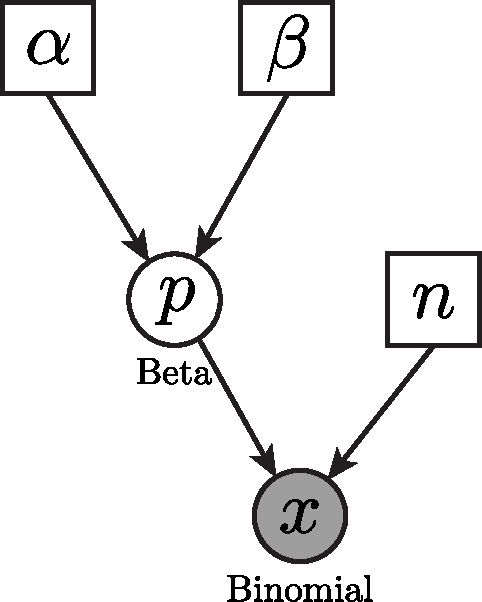
\includegraphics[width=1.8in,angle=0]{\ResourcePath figures/binomial_graphical_model.pdf}}
\label{binomial_model}
\end{figure}

\section{Writing an MCMC from Scratch}
\subsection{The Metropolis-Hastings Algorithm}
Though \RevBayes implements efficient and easy-to-use Markov chain Monte Carlo algorithms, we'll begin by writing one ourselves to gain a better understanding of the moving parts.
The Metropolis-Hastings MCMC algorithm proceeds as follows:

\begin{enumerate}
	\item Generate initial values for the parameters of the model (in this case, $p$).
	\item Propose a new value for some parameters of the model, based on their current values (which we'll call $p^\prime$)
	\item Calculate the acceptance probability, $R$, according to:
	\begin{align*}
		R = \text{min}\left\{1, \frac{P(x \mid p^\prime)}{P(x \mid p)} \times \frac{P(p^\prime)}{P(p)} \times \frac{q(p)}{q(p^\prime)} \right\}
	\end{align*}
	\item Generate a uniform random number between 1 and 0. If it is less than $R$, accept the move (set $p = p^\prime$). Otherwise, keep the current value of $p$.
	\item Return to step 2 many many times, keeping track of the value of $p$.
\end{enumerate}

\subsection{Reading in the data}
Actually, in this case, we're just going to make up some data on the spot.
Feel free to alter these values to see how they influence the posterior distribution
{\tt \begin{snugshade*}
\begin{lstlisting}    
# Make up some coin flips!
# Feel free to change these numbers
n <- 100 # the number of flips
x <- 63	# the number of heads
\end{lstlisting}
\end{snugshade*}}

\subsection{Initializing the Markov chain}
We have to start the MCMC off with some initial parameter values.
One way to do this is to randomly draw values of the parameter (just $p$, in this case) from the prior distribution.
We'll assume a ``flat'' beta distribution; that is, one with parameters $\alpha = 1$ and $\beta = 1$.
{\tt \begin{snugshade*}
\begin{lstlisting}
# Initialize the chain with starting values
alpha = 1
beta  = 1
p <- rbeta(1,alpha,beta)[1]
\end{lstlisting}
\end{snugshade*}}

We also need to initialize the likelihood and prior values.
We use the binomial probability for the likelihood function:
{\tt \begin{snugshade*}
\begin{lstlisting}
# Compute the initial likelihood and prior probabilities
likelihood <- (p^x) * (1-p)^(n-x)
\end{lstlisting}
\end{snugshade*}}
and the beta probability for the prior on $p$:
{\tt \begin{snugshade*}
\begin{lstlisting}    
prior      <- p^(alpha-1) * (1-p)^(beta-1)
\end{lstlisting}
\end{snugshade*}}

We also need to initialize a file into which to write the MCMC samples:
{\tt \begin{snugshade*}
\begin{lstlisting}    
# Prepare a file to log our samples
write("iteration","p","\n",file="binomial_MH.log")
write(0,p,"\n",file="binomial_MH.log",append=TRUE)
\end{lstlisting}
\end{snugshade*}}
(You may have to change the newline characters to \texttt{"$\backslash$r$\backslash$n"} if you're using a Windows operating system.)

\subsection{Writing the MH Algorithm}
At long last, we can write our MCMC algorithm.
We will repeat this resampling procedure many times (here, 10000), and iterate the MCMC using a \texttt{for} loop:
{\tt \begin{snugshade*}
\begin{lstlisting}    
# Write the MH algorithm
reps = 10000
for(rep in 1:reps){
\end{lstlisting}
\end{snugshade*}}
(remember to close your \texttt{for} loop at the end).

The first thing we do in the first generation is generate a new value of $p^\prime$ to evaluate.
We'll propose a new value of $p$ from a narrow uniform distribution centered on the current value.
{\tt \begin{snugshade*}
\begin{lstlisting}    
	# Propose a new value of p
	p_prime <- p + runif(1,-0.1,0.1)[1]
\end{lstlisting}
\end{snugshade*}}
One thing we have to be careful about is making sure $p$ (being a probability) stays between 0 and 1.
We can do that by reflecting any proposals outside of that region back into the valid region.
(One of the nice things about the real MCMC algorithms implemented in \RevBayes is that it takes care of this for us).
{\tt \begin{snugshade*}
\begin{lstlisting}    
	if (p_prime < 0) {
		p_prime <- abs(p_prime)
	} else if (p_prime > 1) {
		p_prime <- 2 - p_prime
	}
\end{lstlisting}
\end{snugshade*}}

Next, we compute the proposed likelihood and prior probabilities, as well as the acceptance probability, $R$:
{\tt \begin{snugshade*}
\begin{lstlisting}    
	# Compute the new likelihood and prior	
	likelihood_prime <- (p_prime^x) * (1-p_prime)^(n-x)
	prior_prime      <- p^(alpha-1) * (1-p)^(beta-1)

	# Compute the acceptance probability
	R <- (likelihood_prime/likelihood) * (prior_prime/prior)
\end{lstlisting}
\end{snugshade*}}

Then, we accept the proposal with probability $R$ and reject otherwise:
{\tt \begin{snugshade*}
\begin{lstlisting}    
	# Accept or reject the proposal
	u <- runif(1,0,1)[1]
	if(u < R){
		# Accept the proposal
		p <- p_prime
		likelihood <- likelihood_prime
		prior <- prior_prime
	}
\end{lstlisting}
\end{snugshade*}}

Finally, we store the current value of $p$ in our log file.
{\tt \begin{snugshade*}
\begin{lstlisting}
	# Write the samples to a file
	write(rep,p,"\n",file="binomial_MH.log",append=TRUE)

} # end MCMC\end{lstlisting}
\end{snugshade*}}

If we execute this script, the \texttt{.log} file will contain samples from the posterior distribution of the model!
We can open the file in \texttt{Tracer} to learn about various features of the posterior distribution, for example: the posterior mean or the 95\% credible interval.
Pretty awesome, right?
However, this MCMC algorithm is \emph{very} specific to our binomial model and thus hard to extend (also it's pretty inefficient!).
We'll now specify the exact same model in \Rev using the built-in modeling functionality.

\section{The Metropolis-Hastings Algorithm with the \emph{Real} \RevBayes}
It turns out that the \Rev code to specify the above model is extremely simple.
Again, we start by ``reading in'' (\emph{i.e.},making up) our data.

{\tt \begin{snugshade*}
\begin{lstlisting}    
# Make up some coin flips!
# Feel free to change these numbers
n <- 100 # the number of flips
x <- 63	# the number of heads
\end{lstlisting}
\end{snugshade*}}

Now we specify our prior model.
{\tt \begin{snugshade*}
\begin{lstlisting}    
# Specify the prior distribution
alpha <- 1
beta  <- 1
p ~ dnBeta(alpha,beta)
\end{lstlisting}
\end{snugshade*}}

One difference between \RevBayes and the MH algorithm that we wrote above is that many MCMC proposals are already built-in, but we have to specify them \emph{before} we run the MCMC.
We usually define (at least) one move per parameter immediately after we specify the prior distribution for that parameter.

{\tt \begin{snugshade*}
\begin{lstlisting}    
# Define a move for our parameter, p
moves[1] = mvSlide(p,delta=0.1)
\end{lstlisting}
\end{snugshade*}}

Next, our likelihood model.
{\tt \begin{snugshade*}
\begin{lstlisting}    
# Specify the likelihood model
k ~ dnBinomial(p, n)
k.clamp(x)
\end{lstlisting}
\end{snugshade*}}

We wrap our full Bayesian model into one model object (this is a convenience to keep the entire model in a single object, and is more useful when we have very large models):
{\tt \begin{snugshade*}
\begin{lstlisting}    
# Construct the full model
my_model = model(p)
\end{lstlisting}
\end{snugshade*}}

We use ``monitors'' to keep track of parameters throughout the MCMC.
The two kinds of monitors we use here are the \texttt{mnModel}, which writes parameters to a specified file, and the \texttt{mnScreen}, which simply outputs some parts of the model to screen (as a sort of progress bar).
{\tt \begin{snugshade*}
\begin{lstlisting}    
# Make the monitors to keep track of the MCMC
monitors[1] = mnModel(filename="binomial_MCMC.log", printgen=10, separator = TAB)
monitors[2] = mnScreen(printgen=100, p)
\end{lstlisting}
\end{snugshade*}}

Finally, we assemble the analysis object (which contains the model, the monitors and the moves), and execute the run using the \texttt{.run} command:
{\tt \begin{snugshade*}
\begin{lstlisting}    
# Make the analysis object
analysis = mcmc(my_model, monitors, moves)

# Run the MCMC
analysis.run(100000)
\end{lstlisting}
\end{snugshade*}}
Open the resulting \texttt{binomial\_MCMC.log} file in \texttt{Tracer}.
Do the posterior distributions for the parameter $p$ look the same as the ones we got from our first analysis?

Hopefully, you'll note that this \Rev model is substantially simpler and easier to read than the MH algorithm script we began with.
Perhaps more importantly, this \Rev analysis is \emph{orders of magnitude} faster than our own script, because it makes use of extremely efficient probability calculations built-in to \RevBayes (rather than the ones we hacked together in our own algorithm).

\subsection{Exercise}
Play around with various parts of the model to develop on intuition for both the Bayesian model and the MCMC algorithm.
For example, how does the posterior distribution change as you increase the number of coin flips (say, increase both the number of flips and the number of heads by an order of magnitude)?
How does the estimated posterior distribution change if you change the prior model parameters, $\alpha$ and $\beta$ (\IE is the model prior sensitive)?
Does the prior sensitivity depend on the sample size?
Are the posterior estimates sensitive to the length of the MCMC?
Do you think this MCMC has been run sufficiently long, or should you run it longer?










